\documentclass[apesctratio=169]{beamer}
\usetheme{Madrid} %More themes in https://hartwork.org/beamer-theme-matrix/ %Madrid
\usecolortheme{whale} %whale
\setbeamercovered{transparent}

\usepackage{multimedia}

\usepackage[utf8]{inputenc}
\usepackage{amsmath,amsfonts,amssymb}
\usepackage{graphicx}
\usepackage{float}
\usepackage[portuguese]{babel}

\title[Termografia da Mama-Séries Temporais]{\textbf{Detecção de Regiões Suspeitas em Termografia da Mama Usando Matrix Profile}}
%\subtitle{Dispositivo de aquisição e acompanhamento de sinais cardíacos}
\author[Gabriel Borralho]{Antonio Gabriel Sousa Borralho. \textcolor{blue}{gsborralho@gmail.com} \\ Jessica P. S. Cardoso (PUC-RJ) \\ Prof. Dr. Stelmo M. B. Netto (UFMA) \\ Prof. Dr. Aristófanes Correa Silva (UFMA) \\ Prof. Dr. Anselmo Cardoso de Paiva (UFMA)}
%\author[Gabriel Borralho]{Antonio Gabriel Sousa Borralho \\ Orientador: Prof. Aristófanes Corrêa Silva \\ \ {\footnotesize\ttfamily gabriel.borralho@hotmail}}
\institute[UFMA]{\textbf{Universidade Federal do Maranhão} \\ Núcleo de Computação Aplicada - NCA \\Laboratório de Processamento e Análise de Imagens - LabPAI}
\date{\today}
\logo{
\includegraphics[scale=0.3]{cbis.jpg}}

\begin{document}
	\begin{frame}
		\titlepage
	\end{frame}
	
	\begin{frame}
		\frametitle{Sumário}
		\tableofcontents%[pausesections]
	\end{frame}

	\section{Introdução}
	    \begin{frame}{Introdução}
	        \begin{block}
	        
	            O câncer da mama é o segundo tipo de câncer mais comum entre mulheres de todo o mundo.
	        \end{block}
	        \begin{block}
	            
	            Somente para o ano de 2018, estimam-se 59.700 novos casos no Brasil.
	        \end{block}
	        \begin{block}
	            
	            O principal motivo é o diagnóstico tardio.
	        \end{block} 
	        
	    \end{frame}
	
	\begin{frame}{Introdução}
	    \begin{block}{Mamografia}
	        \begin{itemize}
	            \item Exames periódicos aumentam a chance de detecção precoce.
	            \item A sensibilidade do exame varia por alguns fatores como: qualidade do exame, experiência do especialista e idade da paciente.
	            \item A mamografia faz uso de radiação.
	        \end{itemize}
	    \end{block} 
	    
	    \begin{block}{Termografia Infravermelha (TI)}
	        \begin{itemize}
	            \item Apresenta baixo custo.
	            \item Registra as temperaturas pela superfície corpórea (não invasivo).
	            \item Detecta problemas no suprimento de sangue.
	        \end{itemize}
	    \end{block}
	    
	\end{frame}
	
	\begin{frame}{Introdução}
	    \begin{block}{Objetivo}
	        Propor uma metodologia para classificação de exames, por meio da análise de TI, em saudável e doente, modelando o problema usando séries temporais.
	    
	    \end{block}
	\end{frame}
	
	\section{Fundamentação Teórica} 
	    \begin{frame}{Fundamentação Teórica}
	        \begin{block}{Características do Câncer}
	             \begin{itemize}
	                 \item A célula tumoral diferencia-se da normal pelo fato de não possuir mais o controle de crescimento.
	                 \item Células tumorais necessitam de nutrientes.
	                 \item Por consequência há um aumento do fluxo sanguíneo na região.
	             \end{itemize}
	        \end{block}
	    \end{frame}
	
    	\begin{frame}{Fundamentação Teórica}
                  Uma série temporal T é uma sequência valores de números reais $t_i$, $T = T_1$, $T_2$, ... $T_n$, onde n é o comprimento de T.
                  
                  \begin{figure}[H]
    			        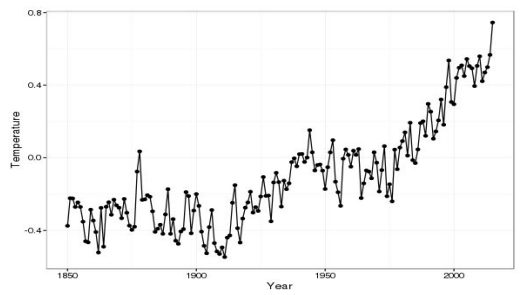
\includegraphics[width=180px, height=100px]{st.PNG}
    			        \caption{Séries temporais}
    		      \end{figure}
        \end{frame}
        
        \begin{frame}{Análise de séries temporais}
            \begin{block}{Descobertas de \textit{Motifs}}
	             \begin{itemize}
	                 \item Padrões desconhecidos e frequentes são denominado \textit{motifs}.
	                 \item Comparação entre subsequências a partir de uma medida de similaridade.
	             \end{itemize}
	        \end{block}
	        
	        \begin{block}{Descobertas de \textit{Discords}}
	             \begin{itemize}
	                 \item Subsequências mais distintas dentro de uma série.
	                 \item Elementos que se destacam na série.
	             \end{itemize}
	        \end{block}
	    \end{frame}
	    
	    \begin{frame}{Análise de séries temporais}
	        
	        \begin{block}{\textit{Matrix Profile}}
	             \begin{itemize}
	                 \item Estrutura de dado que anota uma série temporal.
	                 \item Exato para descoberta de \textit{motifs} e \textit{discords}.
	            \end{itemize}
	        \end{block}
            
	        \begin{figure}[H]
    			     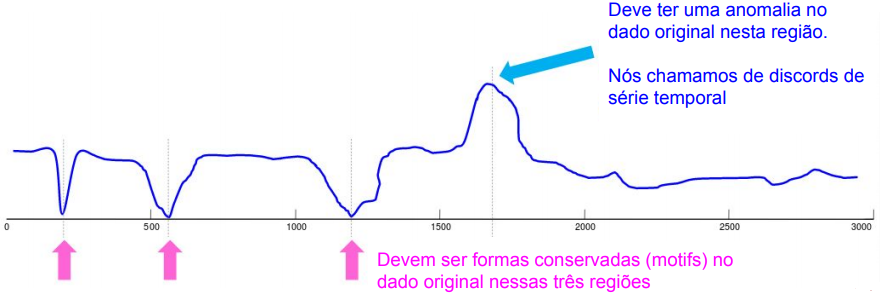
\includegraphics[scale=0.5]{mp.PNG}
    			     \caption{Matrix Profile}
    		\end{figure}
	   \end{frame}
	   
	   \begin{frame}{Fundamentação Teórica}
	        
	        \begin{block}{Máquina de Vetores de Suporte (SVM)}
	             \begin{itemize}
	                 \item Técnica de aprendizagem supervisionada que faz uso da teoria de aprendizado estatístico.
	                 \item Construção de um hiperplano ótimo como superfície de decisão.
	            \end{itemize}
	        \end{block}
            
	        \begin{figure}[H]
    			     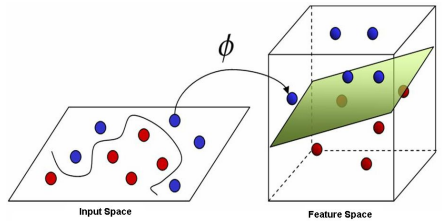
\includegraphics[scale=0.5]{svm.PNG}
    			     \caption{SVM}
    		\end{figure}
	   \end{frame}
	   
	   \begin{frame}{Fundamentação Teórica}
	   Métricas utilizadas para validação dos resultados:
	           \begin{itemize}
	               \item \textbf{Sensibilidade}: $$SE = \dfrac{TP}{TP+FN}$$
	               \item \textbf{Precisão}: $$PR = \dfrac{TP}{TP+FP}$$
	               \item \textbf{Acurácia}: $$AC = \dfrac{TP+TN}{TP+TN+FP+FN}$$
	           \end{itemize}
	       
        TP: séries doentes classificadas corretamente;
                    
        TN: séries saudáveis classificadas corretamente;
                    
        FP: séries saudáveis classificadas como séries doentes;
                    
        FN: séries doentes classificadas como saudáveis;

	   \end{frame}
    
	\section{Metodologia}
	
	\begin{frame}{Metodologia}
	    ETAPAS:
	    
        \begin{figure}[H]
			     
\includegraphics[scale=0.26]{etapas.PNG}
			     \caption{Metodologia proposta}
		\end{figure}
	\end{frame}
	
	\begin{frame}{Metodologia}
	    \begin{block}{1. Aquisição das imagens}
	             \begin{itemize}
	                 \item Processo de \textit{Database for Mastology Research with Infrared Image} (DMR-IR).
	                 \item Pacientes oriundos do Hospital Universitário Antônio Pedro da Universidade Federal Fluminense (HUAPE-UFF).
	                 \item Constituindo 70 exames, sendo 35 saudáveis e 35 doentes.
	                 \item Captura começa após resfriamento do tórax alcançar 30,5º ou 5 minutos.
	                 \item Cada exame é constituído de 20 imagens capturadas a cada 5 segundos por meio de uma câmera térmográfica.
	            \end{itemize}
	        \end{block}
	\end{frame} 
	
    \begin{frame}{1. Aquisição das Imagens}
        \begin{figure}[H]
			     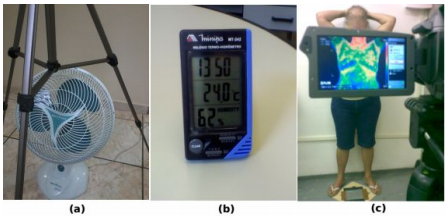
\includegraphics[scale=0.7]{etapa1.PNG}
			     \caption{Aquisição das imagens: a) Aparelho utilizado para resfriamento da região torácica; b) Instrumento de medição da temperatura c) Câmera termográfica}
		\end{figure}
	\end{frame}
	
	\begin{frame}{Metodologia}
	    \begin{block}{2. Pré-processamento}
	             \begin{itemize}
	                 \item Inicialmente, as matrizes de temperatura são convertidas em níveis de cinza.
	                 \item Temperaturas que possuem valores mais altos são representadas com valores de maior intensidade.
	                 \item Valores de temperatura mais baixos irão corresponder a menores intensidades.
	            \end{itemize}
	   \end{block}
	   
	   \begin{block}{3. Segmentação da mama}
	             \begin{itemize}
	                 \item Como o objetivo é buscar por anomalias na região das mamas, é realizada uma segmentação da \textit{Region of Interest} (ROI).
	                 \item Eliminar informações desnecessárias dando origem a uma máscara.
	                 \item Essa operação é feita manualmente por especialistas para cada paciente.
	            \end{itemize}
	   \end{block}
	\end{frame}
	
	\begin{frame}{2. Aquisição das Imagens e 3. Segmentação da mama}
        \begin{figure}[H]
			     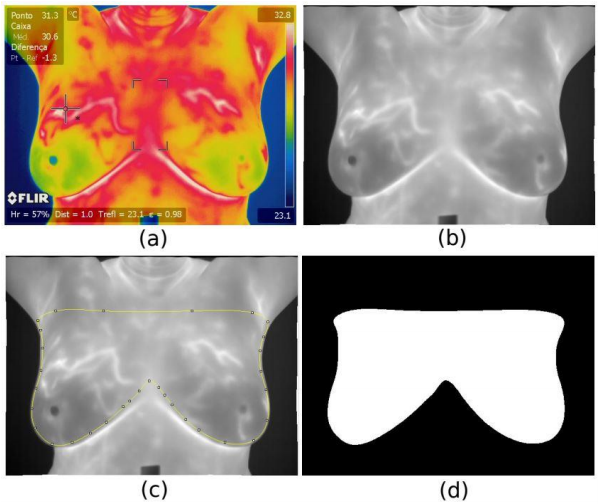
\includegraphics[scale=0.5]{etapa23.PNG}
			     \caption{Aquisição e segmentação das imagens}
		\end{figure}
	\end{frame}
	
	\begin{frame}{Metodologia}
	    \begin{block}{4. Construção das séries}
	             \begin{itemize}
	                 \item A máscara é dividida em uma matriz quadrada de quadrados de mesmo tamanho.
	                 \item A temperatura média de cada quadrado é observada em todos os vinte termogramas de cada paciente, produzindo a série temporal.
	            \end{itemize}
	   \end{block}
	   
	   \begin{figure}[H]
			     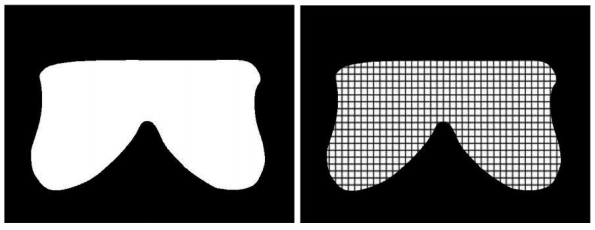
\includegraphics[scale=0.5]{etapa4.PNG}
			     \caption{Janelamento}
		\end{figure}
	\end{frame}
	
	\begin{frame}{4. Construção das séries}
        \begin{figure}[H]
			     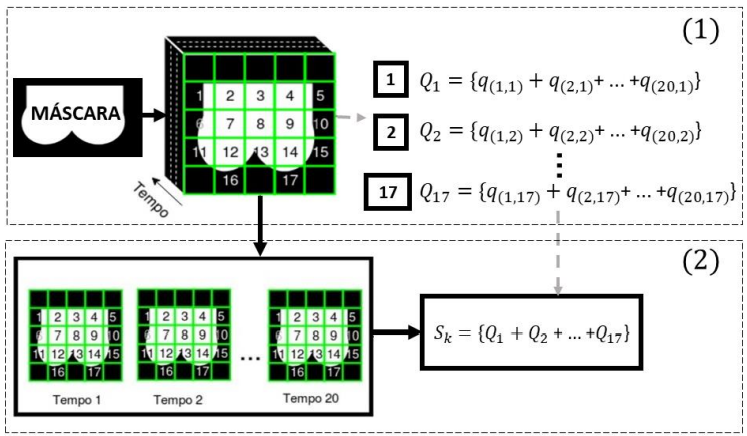
\includegraphics[scale=0.5]{etapa41.PNG}
			     \caption{Construção das séries temporais}
		\end{figure}
	\end{frame}
	
	\begin{frame}{5. Extração de Características}
	    
      \begin{figure}[H]
        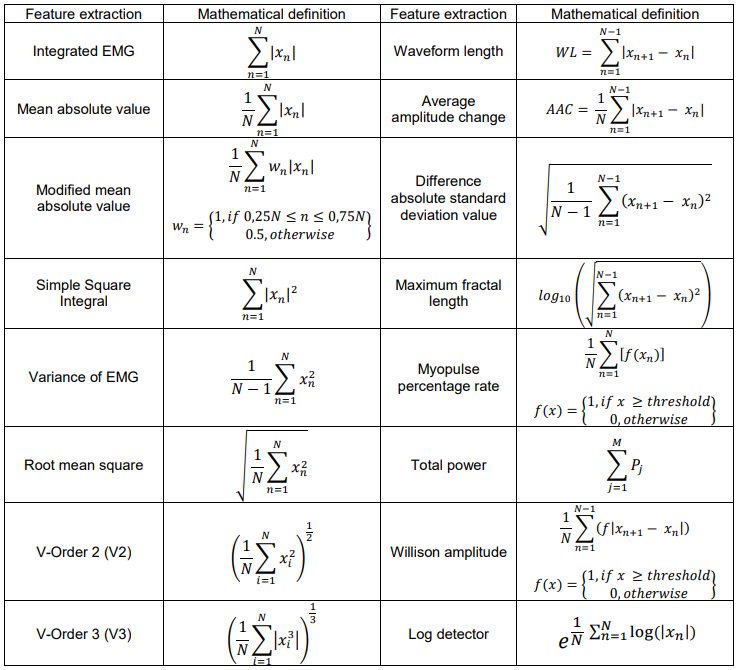
\includegraphics[scale=0.3]{feat.PNG}
        \caption{Sugeridas por "Applications, Challenges, and Advancements in Electromyography Signal Processing" (Ganesh, R. Naik)}
      \end{figure}
      
	\end{frame}
	
	\begin{frame}{Aplicação do Matrix Profile}
        \begin{figure}[htb]
			     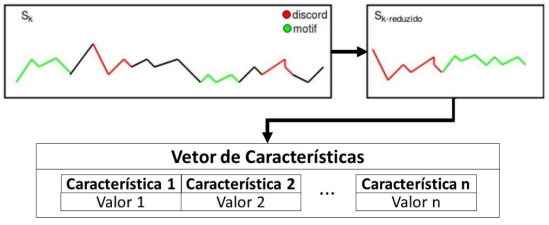
\includegraphics[scale=0.5]{etapa5.PNG}
			     \caption{Extração de Características}
		\end{figure}
	\end{frame}
	
	\begin{frame}{Metodologia}
	    \begin{block}{6. Classificação}
	             \begin{itemize}
	                 \item Classes: doente e saudáveis.
	                 \item SVM como método de aprendizagem supervisionada.
	                 \item Para a tarefa de classificação, foi utilizada a biblioteca LIBSVM.
	                 \item Foi realizado um treino 35/35
	                 \item Foi utilizado validação cruzada de 5-folds.
	            \end{itemize}
	   \end{block}
	\end{frame}
	
	\section{Resultados}
	
	\begin{frame}{Resultados}
	\begin{block}{Os testes foram realizados de quatro maneiras:}
	             \begin{itemize}
	                 \item  (1) série gerada antes da utilização do \textit{Matrix Profile}; 
	                 \item  (2) série gerada pela concatenação de \textit{motifs}; 
	                 \item  (3) série gerada pela concatenação de \textit{discords};
	                 \item  (4) série obtida a partir da união de motifs e discords;
	            \end{itemize}
	\end{block}
	
	\end{frame}
	
	\begin{frame}{Resultados}
        \begin{figure}[htb]
			     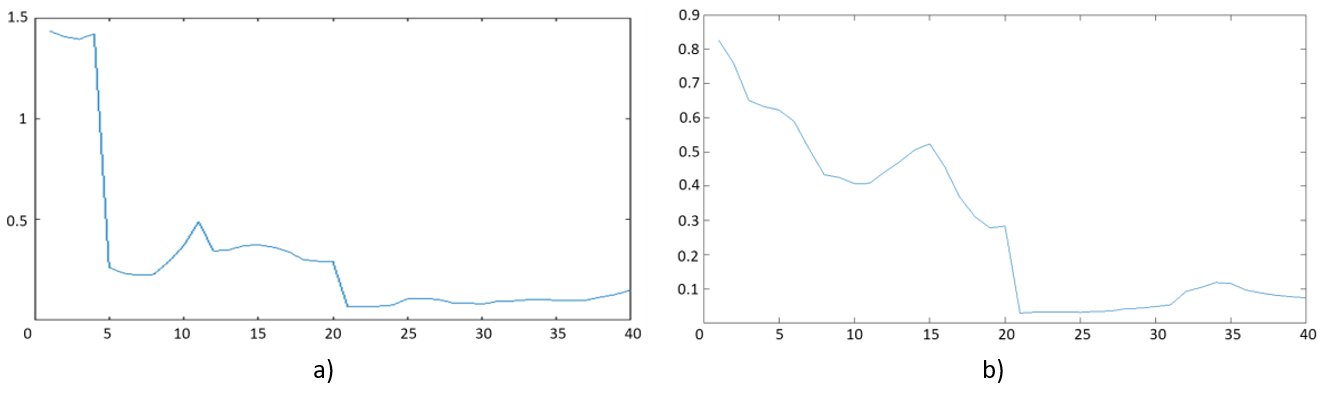
\includegraphics[scale=0.35]{result.PNG}
			     \caption{Série de uma paciente: a)doente e b)saudável}
		\end{figure}
	\end{frame}
	
	\begin{frame}{Resultados}
        \begin{figure}[htb]
			     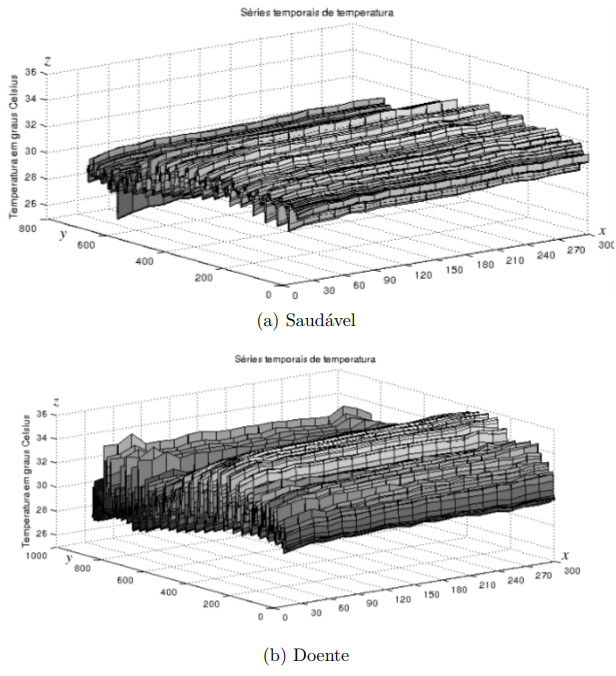
\includegraphics[scale=0.4]{series.PNG}
			     %\caption{Conjunto de séries de uma paciente: a)doente e b)saudável}
		\end{figure}
	\end{frame}
	
	
	\begin{frame}{Resultados}
	    Métricas utilizadas: Acurácia (AC), Sensibilidade(SE) e Precisão (PR).
	    \begin{table}[htb]
        	\centering
        	\begin{tabular}{c|c|c|c}
        		\hline		
        	    Método & $AC_{med}$ & $SE_{med}$ & $PR_{med}$\\
        		\hline
        		Antes do \textit{Matrix Profile} & $74,29\%$ & $75,60\%$ & $71,43\%$\\
        		\hline
        		Apenas com $motifs$ & $62.86\%$ & $70,59\%$ & $60,00\%$\\
        		\hline
        		\textbf{Apenas com \textit{discords}} & \textbf{87,14\%} & \textbf{87,50\%} & \textbf{84,85\%}\\
        		\hline
        		União de $motifs$ e $discords$ & $82,86\%$ & $80,00\%$ & $84,85\%$\\
        		\hline
        	\end{tabular}
        	\caption{Resultados obtidos}
        	\label{tabela-1}
        \end{table}
	\end{frame}
	
	\section{Conclusão}
	\begin{frame}{Conclusão}
	
	    \begin{block}
	    
	        \begin{itemize}
	            \item Diagnóstico precoce aumenta a chance de sobrevida.
	            \item  A distinção entre pacientes saudáveis e doentes são visíveis.
	            \item  Nos 20 primeiros valores, que representam os \textit{discords}, a diferença é notória.
	            \item  \textit{motifs} não são tão eficazes para serem utilizados como instrumento para classificação.
	        \end{itemize}
	    \end{block}
	\end{frame}
	
	\section{Trabalhos Futuros}
	
	\begin{frame}{Trabalhos Futuros}
	    \begin{itemize}
	        \item Pretende-se testar outras maneiras de realizar a construção das séries temporais como, por exemplo, utilizar os valores máximos de temperatura para a construção das séries;
	        \item Utilização de outras técnicas de reconhecimento de padrões;
	        \item Geração de séries sintéticas;
	        \item Aumentar a base de exames de termografias;
	        \item Segmentação automática;
	    \end{itemize}
	    
	\end{frame}
	
	\begin{frame}{Agradecimentos}
	    \begin{figure}[htb]
			     
\includegraphics[scale=0.35]{ak.PNG}
		\end{figure}
	\end{frame}		
	
\end{document}